\documentclass[a4paper,14pt]{extarticle}

\usepackage[T2A]{fontenc}
\usepackage[utf8]{inputenc}
\usepackage[russian]{babel}
\usepackage{geometry}
\usepackage{setspace}
\usepackage{indentfirst}
\usepackage{array}
\usepackage{booktabs}
\usepackage{listings}
\usepackage{xcolor}
\usepackage{graphicx}
\usepackage{float}

\geometry{
    left=30mm,
    right=15mm,
    top=20mm,
    bottom=20mm
}

\onehalfspacing
\setlength{\parindent}{1.25cm}
\setlength{\parskip}{0pt}

\definecolor{codebg}{RGB}{248,248,248}
\lstdefinestyle{cudastyle}{
    language=C++,
    basicstyle=\ttfamily\normalsize,
    keywordstyle=\color{blue!60!black},
    commentstyle=\color{green!40!black},
    stringstyle=\color{orange!50!black},
    backgroundcolor=\color{codebg},
    frame=single,
    breaklines=true,
    showstringspaces=false,
    tabsize=4
}

\begin{document}

\begin{titlepage}
    \begin{center}
        \textbf{МОСКОВСКИЙ АВИАЦИОННЫЙ ИНСТИТУТ}\\
        \textbf{(НАЦИОНАЛЬНЫЙ ИССЛЕДОВАТЕЛЬСКИЙ УНИВЕРСИТЕТ)}\\
        Институт №8 «Компьютерные науки и прикладная математика»
    \end{center}

    \vspace{3.5cm}

    \begin{center}
        \textbf{\Large Лабораторная работа №2}\\
        \vspace{0.3cm}
        по курсу «Технологии параллельного программирования»\\
        \vspace{0.8cm}
        \textbf{Обработка изображений на GPU. Фильтры.}
    \end{center}

    \vspace{4cm}

    \begin{flushright}
        Выполнил: Ахметшин Б.Р.\\
        Группа: М8О-403Б-22\\
        Преподаватели: А.Ю. Морозов,\\
        \hspace*{3.6cm} Е.Е. Заяц
    \end{flushright}

    \vfill

    \begin{center}
        Москва, 2026
    \end{center}
\end{titlepage}

\section*{Условие}
Цель работы: научиться использовать GPU для обработки изображений.
Использование текстурной памяти и двухмерной сетки потоков.

Выполненная реализация: фильтр выделения границ Превитта для изображения
в пользовательском бинарном формате (\texttt{w}, \texttt{h}, затем пиксели \texttt{rgba}).

\section*{Программное и аппаратное обеспечение}
\textbf{GPU}

\begin{tabular}{>{\raggedright\arraybackslash}p{0.50\textwidth}>{\raggedright\arraybackslash}p{0.34\textwidth}}
Имя & NVIDIA Tesla T4 \\
Compute Capability & 7.5 \\
Объем глобальной памяти & 15637086208 \\
Разделяемая память на блок & 49152 \\
Константная память & 65536 \\
Регистров на блок & 65536 \\
Макс. потоков на блок & (1024, 1024, 64) \\
Макс. размер сетки & (2147483647, 65535, 65535) \\
Количество мультипроцессоров & 40 \\
\end{tabular}

\vspace{0.4cm}
\textbf{CPU}

\begin{tabular}{>{\raggedright\arraybackslash}p{0.50\textwidth}>{\raggedright\arraybackslash}p{0.34\textwidth}}
Архитектура & x86\_64 \\
CPU op-mode(s) & 32-bit, 64-bit \\
Address sizes & 48 bits physical, 48 bits virtual \\
Порядок байт & Little Endian \\
CPU(s) & 12 \\
Имя модели & AMD Ryzen 5 7600 6-Core Processor \\
Ядер / потоков & 6 / 12 \\
\end{tabular}

\vspace{0.4cm}
\textbf{RAM}\\
64 GB

\vspace{0.2cm}
\textbf{ОС}\\
Ubuntu 24.04.4 LTS

\vspace{0.2cm}
\textbf{Компилятор}\\
nvcc, g++

\section*{Метод решения}
Изображение читается в массив \texttt{uchar4} (rgba), после чего копируется в
\texttt{cudaArray} и связывается с \texttt{cudaTextureObject}. Ядро запускается на двумерной
сетке потоков (блок \texttt{16x16}), каждый поток обрабатывает один пиксель.

Для вычисления интенсивности используется перевод в оттенок серого:
\[
gray = 0.299r + 0.587g + 0.114b.
\]
Далее применяются маски Превитта по осям \texttt{x} и \texttt{y}; итоговая величина
градиента:
\[
g = \sqrt{g_x^2 + g_y^2},
\]
после чего значение ограничивается диапазоном \([0,255]\) и записывается в
выходной пиксель как \texttt{r=g=b=g}, \texttt{a=0}.

\section*{Описание программы}
Файлы реализации:
\begin{itemize}
    \item \texttt{lab2.cu} --- GPU-реализация на CUDA;
    \item \texttt{lab2-cpu.cpp} --- CPU-реализация для сравнения;
    \item \texttt{converter.py} --- конвертация между бинарным форматом ЛР и PNG.
\end{itemize}

В GPU-версии реализованы два вида измерений:
\begin{itemize}
    \item \texttt{kernel\_ms} --- время ядра (через CUDA events);
    \item \texttt{total\_ms} --- совокупное время вычислительной части
    (от старта GPU-обработки до получения результата на CPU).
\end{itemize}
Оба значения логируются в файл \texttt{timings\_gpu\_lab2.txt} (или путь из переменной
\texttt{LAB2\_TIMING\_FILE}).

CPU-версия логирует \texttt{total\_ms} в файл \texttt{timings\_cpu\_lab2.txt}
(или путь из \texttt{LAB2\_TIMING\_FILE}).

Сборка:
\begin{lstlisting}[style=cudastyle]
cd lab2
make
\end{lstlisting}

Запуск (GPU):
\begin{lstlisting}[style=cudastyle]
printf "in.data\nout_gpu.data\n" | ./lab2
\end{lstlisting}

Запуск (CPU):
\begin{lstlisting}[style=cudastyle]
printf "in.data\nout_cpu.data\n" | ./lab2-cpu
\end{lstlisting}

\section*{Результаты}
\textbf{Замеры:}

\begin{lstlisting}[basicstyle=\ttfamily\scriptsize,frame=single]
+----+-----------+--------------------------+------------+----------------+---------------+
| No | image     | CUDA (grid, block)       | CPU, ms    | GPU kernel, ms | GPU total, ms |
+----+-----------+--------------------------+------------+----------------+---------------+
| 1  | 512x512   | <<<(64x64), (8x8)>>>     | 6.100761   | 0.134752       | 384.695764    |
| 2  | 512x512   | <<<(32x32), (16x16)>>>   |            | 0.141344       | 382.040485    |
| 3  | 512x512   | <<<(16x64), (32x8)>>>    |            | 0.138944       | 381.365321    |
| 4  | 4096x4096 | <<<(512x512), (8x8)>>>   | 436.016163 | 1.592064       | 462.457037    |
| 5  | 4096x4096 | <<<(256x256), (16x16)>>> |            | 1.961760       | 502.916248    |
| 6  | 4096x4096 | <<<(128x512), (32x8)>>>  |            | 1.838432       | 463.340353    |
+----+-----------+--------------------------+------------+----------------+---------------+
\end{lstlisting}

\textbf{Скриншоты (обязательное требование для ЛР2):}

\begin{figure}[H]
    \centering
    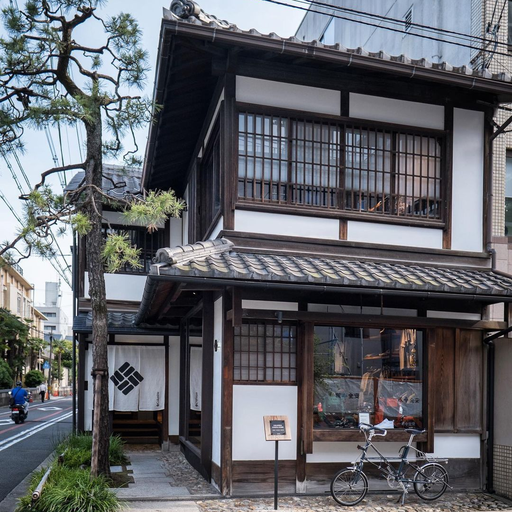
\includegraphics[width=0.47\textwidth]{images/pic1_512x512.png}
    \hfill
    \includegraphics[width=0.47\textwidth]{images/pic1_512x512_out.png}
    \caption{Визуальное сравнение до и после обработки}
\end{figure}

\section*{Выводы}
В лабораторной работе реализован фильтр обработки изображений на GPU
с использованием текстурной памяти и двумерной сетки потоков, а также
эквивалентная CPU-реализация для сравнения производительности.

По замерам видно, что время ядра GPU мало и хорошо масштабируется:
для изображения \(512\times512\) оно составляет \(0.134\mbox{--}0.141\) мс,
а для \(4096\times4096\) --- \(1.59\mbox{--}1.96\) мс.
Однако совокупное время GPU значительно выше из-за накладных расходов
(копирование данных и служебные операции): \(381\mbox{--}385\) мс для \(512\times512\)
и \(462\mbox{--}503\) мс для \(4096\times4096\).

Сравнение с CPU показывает, что в текущей постановке CPU быстрее по общему времени:
\(6.10\) мс против \(381\mbox{--}385\) мс для \(512\times512\),
и \(436.02\) мс против \(462\mbox{--}503\) мс для \(4096\times4096\).
При этом по времени самого ядра GPU значительно эффективнее, что подтверждает
корректность распараллеливания, но также показывает доминирование накладных расходов
в полном времени выполнения.

Лучшая конфигурация по общему времени:
для \(512\times512\) --- \verb|<<<16x64, 32x8>>>|,
для \(4096\times4096\) --- \verb|<<<512x512, 8x8>>>|.

\end{document}
